\stepcounter{footnote}\newcounter{pizzachili}\setcounter{pizzachili}{\value{footnote}}
\stepcounter{footnote}\newcounter{xmldata}\setcounter{xmldata}{\value{footnote}}
\setlength{\tabcolsep}{3pt}
\begin{table*}[ht]
  \centering
  \begin{tabular}{crrrrrrrrrrrrrrr}
    & \multicolumn{3}{c}{xml} & \multicolumn{3}{c}{dna} & \multicolumn{3}{c}{psd7003} & \multicolumn{3}{c}{protein} & \multicolumn{3}{c}{comptree}\\
    &  \multicolumn{3}{c}{(23,551,472)} & \multicolumn{3}{c}{(32,747,474)} & \multicolumn{3}{c}{(42,611,636)} & \multicolumn{3}{c}{(60,160,372)} & \multicolumn{3}{c}{(2,147,483,646)}\\
\hline
    $p$ & \verb|psta| & \verb|libcds| & \verb|sdsl|  & \verb|psta| & \verb|libcds| & \verb|sdsl| & \verb|psta| & \verb|libcds| & \verb|sdsl| & \verb|psta| & \verb|libcds| & \verb|sdsl| & \verb|psta| & \verb|libcds| & \verb|sdsl|\\
\hline
 1   &  .99  &  9.95  & .60  &  1.01 & 10.68  & .64  &  1.04  & 10.73  & .63  &  .99   &  10.16  &  .61   & 1.00  & 11.59  & .69   \\
 2   &  1.96 &  19.71 & 1.19 &  1.98 & 21.01  & 1.27 &  2.06  & 21.33  & 1.26 &  1.98  &  20.26  &  1.22  & 1.98  & 22.93  & 1.36  \\
 4   &  3.77 &  38.00 & 2.30 &  3.88 & 41.18  & 2.48 &  3.94  & 40.84  & 2.41 &  3.92  &  39.99  &  2.41  & 3.82  & 44.33  & 2.62  \\
 6   &  5.25 &  52.84 & 3.20 &  5.43 & 57.73  & 3.48 &  5.63  & 58.30  & 3.44 &  5.46  &  55.77  &  3.36  & 5.50  & 63.82  & 3.78  \\
 8   &  7.14 &  71.89 & 4.36 &  7.30 & 77.58  & 4.67 &  6.89  & 71.36  & 4.21 &  7.49  &  76.45  &  4.60  & 7.64  & 88.64  & 5.25  \\
 10  &  8.09 &  81.46 & 4.94 &  8.42 & 89.43  & 5.39 &  6.72  & 69.66  & 4.11 &  7.14  &  72.97  &  4.39  & 9.14  & 106.01 & 6.28  \\
 12  &  7.58 &  76.38 & 4.63 &  7.83 & 83.19  & 5.01 &  7.97  & 82.59  & 4.87 &  9.56  &  97.62  &  5.88  & 10.54 & 122.26 & 7.24  \\
 14  &  8.28 &  83.36 & 5.05 &  8.39 & 89.18  & 5.37 &  8.74  & 90.63  & 5.34 &  9.36  &  95.64  &  5.76  & 11.94 & 138.47 & 8.20  \\
 16  &  7.08 &  71.34 & 4.32 &  8.41 & 89.39  & 5.38 &  7.52  & 77.90  & 4.59 &  8.48  &  86.57  &  5.21  & 14.20 & 164.75 & 9.75  \\
\hline\hline
 18  &  7.23 &  72.77 & 4.41 &  5.76 & 61.23  & 3.69 &  10.19 & 105.59 & 6.22 &  9.36  &  95.61  &  5.76  & 14.91 & 172.99 & 10.24\\
 20  &  7.18 &  72.30 & 4.38 &  8.41 & 89.37  & 5.38 &  8.30  & 85.99  & 5.07 &  11.86 &  121.10 &  7.29  & 15.93 & 184.85 & 10.94\\
 22  &  7.43 &  74.84 & 4.53 &  7.69 & 81.72  & 4.92 &  7.98  & 82.75  & 4.88 &  7.83  &  79.99  &  4.82  & 17.20 & 199.60 & 11.82\\
 24  &  5.75 &  57.89 & 3.51 &  7.16 & 76.10  & 4.58 &  9.31  & 96.53  & 5.69 &  9.73  &  99.35  &  5.98  & 17.68 & 205.17 & 12.15\\
 26  &  6.74 &  67.88 & 4.11 &  8.82 & 93.69  & 5.64 &  9.18  & 95.09  & 5.60 &  11.00 &  112.38 &  6.77  & 18.58 & 215.54 & 12.76\\
 28  &  4.48 &  45.09 & 2.73 &  5.80 & 61.62  & 3.71 &  5.59  & 57.98  & 3.42 &  6.54  &  66.76  &  4.02  & 19.31 & 224.00 & 13.26\\
 30  &  4.91 &  49.49 & 3.00 &  9.81 & 104.26 & 6.2  &  6.25  & 64.81  & 3.82 &  8.95  &  91.41  &  5.50  & 19.17 & 222.38 & 13.17\\
 32  &  3.51 &  35.30 & 2.14 &  5.06 & 53.78  & 3.24 &  6.60  & 68.41  & 4.03 &  5.82  &  59.47  &  3.58  & 19.28 & 223.67 & 13.24\\
 \hline
\end{tabular}
\caption[]{Relative speed-up achieved on different data sets using our {\tt PSTA}
  algorithm compared to {\tt PSTA} on a single processor, {\tt libcds}, and {\tt
    sdsl}, respectively.
  The latter two are sequential algorithms.
  This speed-up is the running time of the respective comparator algorithm
  divided by the running time of {\tt PSTA} on the number of processors listed
  in the leftmost column.
  The data sets were LZ78 parsings of the XML ({\tt xml}), DNA ({\tt dna}), and
  protein ({\tt protein}) data from the Pizza \& Chili
  corpus\footnotemark[\value{pizzachili}], as well as data from the XMLData
  repository\footnotemark[\value{xmldata}] ({\tt psd7003}) and a complete binary tree of
  depth 30 ({\tt comptree}).
  The number of parentheses in the input, which is twice the number of nodes in
  the tree, is listed in parentheses for each data set.}
\label{tbl:speedup}
\end{table*}

Table~\ref{tbl:speedup} shows the relative speed-up results obtained by our
{\tt PSTA} algorithm.
Also see Figure~\ref{fig:speedup} for a graphical representation.
We repeated each experiment three times and recorded the minimum running time,
assuming that slightly larger values of any given experiment are just ``noise''
from external processes such as operating system and networking
tasks.\Norbert{One can often argue that the opposite is the case: When the cache
  is already primed, you often see better performance than on an unprimed cache.
  So the right way of doing this is to run each experiment 3 times, but not 3
  times in a row, to avoid cache priming.}

\begin{figure}[ht]
  \centering
  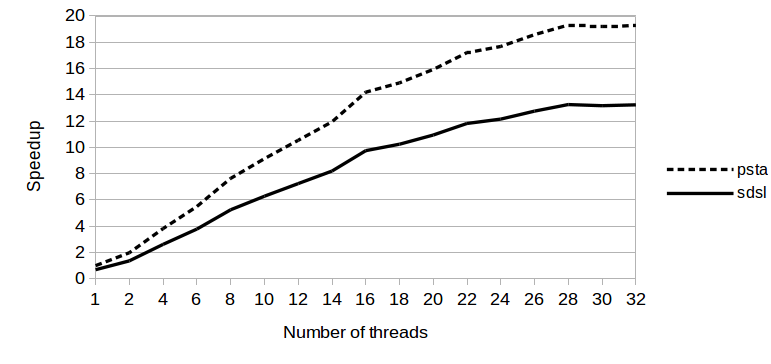
\includegraphics[scale=0.3]{./images/Speedup.png}
  \caption{Speedup of comptree corpus}
  \label{fig:speedup}
\end{figure}

First note that {\tt psta} outperformed {\tt libcds} by an order of magnitude
even on a single core.
As we allowed {\tt psta} to utilize more cores, its advantage over
{\tt libcds} only increased because {\tt libcds} is a purely sequential
program.
{\tt sdsl} was about 1.5 times faster than {\tt psta} on a single core, but
already using two cores {\tt psta} started to be faster than {\tt sdsl}, again
because {\tt sdsl} is a purely sequential program.
The advantage of {\tt sdsl} over {\tt psta} on a single core, in spite of
implementing essentially the same algorithm, can be attributed to (1)
lack of tuning of {\tt psta} and (2) some overhead with running parallel
code on a single core, which {\tt sdsl} avoids by being a purely sequential
program.

Up to 16 cores, the speed-up is almost linear whenever $p$ is a power of $2$,
with an efficiency of 60\%, which is quite good for multicore architectures.
When $p$ is not a power of $2$, speed-up is slightly worse.
The reason is that, when $p$ is a power of $2$, {\tt psta} can assign
exactly one subtree per thread (see Algorithm \ref{algo:PSTA2}),
distributing the work homogeneously across cores and thus not requiring
any work stealing.
When the number of threads is not a power of two, some threads have to process
more than one subtree and other threads process only one, which degrades
performance.  Nevertheless, due to work stealing, no core sits idle for
long and the slight performance degradation is due to the overhead of work
stealing.\Norbert{I made this up.  Does this make sense?  Essentially, the
way it was phrased before doesn't really offer a lot of insight into where
the performance degradation really comes from when the work is not distributed
evenly, and what I wrote here at least matches that we point out that no work
stealing is required when $p = 2^x$.}
For $p = 32$, the efficiency of {\tt psta} drops below 50\%.
This is likely because, on our 32-core machine, less than 32 threads can execute
on their own dedicated cores without interfering with OS processes, which can
run on the 32nd core.
When using 32 threads, the threads of our program start to compete with OS
processes for the available cores, which degrades performance.

The general performance degradation beyond 16 threads is most likely due
to the architecture of the machine we ran our experiments on.
The 4 processors on this machine are arranged in a grid
topology~\cite{Drepper2007}.
Up to 8 threads, communication between the threads is limited to a single
processor running these threads, with very little overhead.
Between 8 and 16 threads require the use of two adjacent processors in
the grid, which still keeps communication cost low.
Beyond 16 threads, three or four processors are needed and at least two
of these processors are not adjacent in the grid, which increases the
communication between the threads on these processors noticeably.
\Leo{Review Drepper's explanation of this}.

Since {\tt psta} generates tasks that work on different memory
regions, the generated cache misses \Leo{false sharing is misses} do
not degrade the performance. The same effect is present on
\emph{Domain Decomposition Algorithms}. Although the decomposition of
the {\tt RMMT} was not evident, we could produce a decomposition that
generated a competitive algorithm.\Norbert{I'm not sure what exactly
you're saying here.  Are you saying that, if the threads were working on the
same memory regions, maintaining cache coherence would essentially force
a lot of reads from RAM because pages in cache become invalid due to writes
by other processors, and given that all our threads work on different memory
regions, this issue does not arise?}
	
\begin{table}[ht]
  \centering
  \begin{tabular}{crrrrr}
\hline
    & xml & dna & psd7003 & protein & comptree\\
\hline
 \verb|psta|   &  1.46  &  1.74  & 2.78  &  3.30 & 112.01\\
 \verb|libcds|   &  .42 &  .58 & .77 &  1.08 & 38.25\\
 \verb|sdsl|   &  .95 &  1.31 & 1.73 &  2.41 & 76.40\\
 \hline
\end{tabular}
\caption{Peak memory consumption of the three algorithms on the data sets
  from Table~\ref{tbl:speedup}, measured in MB.}
\label{tbl:memory_consumption}
\end{table}

Table \ref{tbl:memory_consumption} shows memory consumption for the
corpora usid in our experiments.
For {\tt psta}, the consumption of the single-threaded code ($p = 1$)
is shown.
The extra memory needed for thread scheduling when $p > 1$ was negligible.
To measure memory consumption, we
monitored how much memory was allocated with \texttt{malloc} and
released with \texttt{free} at execution time and recorded the peak
consumption.
We only measured memory allocated during construction of the data structure,
which does not include  the memory allocated to store the parenthesis sequence.
Even though {\tt psta} consumes more memory than both {\tt libcds} and
{\tt sdsl}, the difference between {\tt psta} and {\tt sdsl} is a factor of
less than two.
The difference between {\tt psta} and {\tt libcds} is no more than a factor of
four and is outweighed by the substantially worse performance of {\tt libcds},
even compared to the single-threaded version of {\tt psta}.
More importantly, a memory consumption of 112MB for processing a 1-billion-node
tree amounts to less than one bit per node and, so {\tt psta} can be considered
very space-efficient.

\footnotetext[\value{pizzachili}]{\url{http://pizzachili.dcc.uchile.cl}}
\footnotetext[\value{xmldata}]{\url{http://www.cs.washington.edu/research/xmldatasets}}

Part of the higher memory consumption of {\tt psta} compared to {\tt libcds}
and {\tt sdsl} stems from the allocation of
$e^{\prime}$, $m^{\prime}$, $M^{\prime}$ and $n^{\prime}$ arrays to store the
partial excess values in the algorithm.
Storing these values is a key factor that helps {\tt psta} to achieve very
good performance.
Our implementation allocates 16 bits per excess value in these arrays.
It would be possible to use a simplification
of Algorithm \ref{algo:PSTA1} to calculate the depth $d$ of the input
sequence (the maximum excess value) and then allocate only $\lg d$ bits per
excess value to reduce the space overhead of storing these areas and improve
performance further by reducing the memory bandwidth required to read and write
these arrays.
